\documentclass[12pt]{article}

\usepackage{graphicx}
\usepackage[margin=1in]{geometry} 
\usepackage{amsmath,amsthm,amssymb}

\begin{document}
	
	\title{2D Inverted Pendulum}
	\author{Davis Benz\\
		    Equations of Motion}
	
	\maketitle
	
	\section{Terms}
		\begin{itemize}
			\item Constants
				\begin{itemize}
					\item g: gravity
					\item Itot: total mass moment of inertia of the inverted pendulum
					\item Im: mass moment of inertia of the just rotor
					\item Ib: mass moment of inertia of just the body
					\item m: mass of the related system
				\end{itemize}
			\item Variables
				\begin{itemize}
					\item omega
				\end{itemize}
			\item Subscripts
			\begin{itemize}
				\item \textbf{b}: body
				\item \textbf{m}: motor
				\item \textbf{g}: gravity, IE a force or moment due strictly to gravity
				\item \textbf{f}: friction, frictional forces or moments
				\item \textbf{o}: origin point of the system
			\end{itemize}
		\end{itemize}
	\section{2D System}
		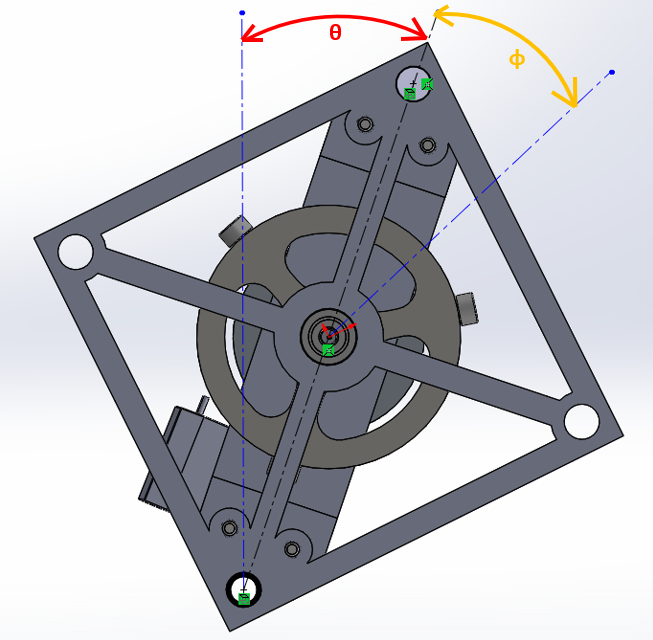
\includegraphics[width=\textwidth]{EoM_Image.png}
	\section{Lagrangian Equation of Motion}
		\subsection{Lagrangian}
			\begin{equation}
				\mathcal{L} = \frac{1}{2}I_b\omega_b^2  +  \frac{1}{2}I_m(\omega_b + \omega_m)^2 - m_{t}gcos(\theta)
			\end{equation}
			\begin{equation}
				\mathcal{L} = \frac{1}{2}I_b\dot\theta^2  +  \frac{1}{2}I_m(\dot\theta + \dot\phi)^2 - m_{t}gcos(\theta)
			\end{equation}
		\subsection{Lagrangian Momentum}
			\begin{equation}
				p_{\theta} = \frac{\sigma\mathcal{L}}{\sigma \dot\theta}
			\end{equation}
			\begin{equation}
				p_{\phi} = \frac{\sigma\mathcal{L}}{\sigma \dot\phi}
			\end{equation}
			\begin{equation}
				\mathcal{L} = \frac{1}{2}I_b\dot\theta^2  +  \frac{1}{2}I_m(\dot\theta^2 + 2\dot\theta\dot\phi + \dot\phi^2) - m_{t}gcos(\theta)
			\end{equation}
			\begin{equation}
				\mathcal{L} = \frac{1}{2}I_b\dot\theta^2  +  \frac{1}{2}I_m\dot\theta^2 + \frac{2}{2}I_m\dot\theta\dot\phi + \frac{1}{2}I_m\dot\phi^2 - m_{t}gcos(\theta)
			\end{equation}
			\begin{equation}
				\frac{\sigma\mathcal{L}}{\sigma \dot\theta} = I_b\dot\theta + I_m\dot\theta + I_m\dot\phi
			\end{equation}
			\begin{equation}
				\frac{\sigma\mathcal{L}}{\sigma \dot\theta} = \dot\theta(I_b + I_m) + I_m\dot\phi, \; I_b = I_{tot} - I_m
			\end{equation}
			\begin{equation}
				\frac{\sigma\mathcal{L}}{\sigma \dot\theta} = \dot\theta(I_{tot} - I_m + I_m) + I_m\dot\phi
			\end{equation}
			\begin{equation}
				\frac{\sigma\mathcal{L}}{\sigma \dot\theta} = I_{tot}\dot\theta + I_m\dot\phi
			\end{equation}
			\begin{equation}
				\frac{\sigma\mathcal{L}}{\sigma \dot\phi} = I_m\dot\theta + I_m\dot\phi
			\end{equation}
			\begin{equation}
				\frac{\sigma\mathcal{L}}{\sigma \dot\phi} = I_m(\dot\theta + \dot\phi)
			\end{equation}
			\begin{equation}
				\boxed{P_\theta = I_{tot}\dot\theta + I_m\dot\phi}
			\end{equation}
			\begin{equation}
				\boxed{P_\phi = I_m(\dot\theta + \dot\phi)}
			\end{equation}
		\subsection{Equations of Motion}
			\begin{equation}
				\frac{d}{dt}\frac{\sigma\mathcal{L}}{\sigma\dot\theta} = \frac{\sigma\mathcal{L}}{\sigma\theta} => \frac{d}{dt}P_\theta = \frac{\sigma\mathcal{L}}{\sigma\theta}
			\end{equation}
			\begin{equation}
				\frac{d}{dt}(I_{tot}\dot\theta + I_m\dot\phi) = m_tgsin(\theta)
			\end{equation}
			\begin{equation}
				I_{tot}\ddot\theta + I_m\ddot\phi = m_tgsin(\theta)
			\end{equation}
			\begin{equation}
				\frac{d}{dt}\frac{\sigma\mathcal{L}}{\sigma\dot\phi} = \frac{\sigma\mathcal{L}}{\sigma\phi} => \frac{d}{dt}P_\phi = \frac{\sigma\mathcal{L}}{\sigma\phi}
			\end{equation}
			\begin{equation}
				\frac{d}{dt}(I_m(\dot\theta + \dot\phi)) = T
			\end{equation}
			\begin{equation}
				I_m(\ddot\theta + \ddot\phi) = T
			\end{equation}
			\begin{equation}
				\boxed{I_{tot}\ddot\theta + I_m\ddot\phi = m_tgsin(\theta)}
			\end{equation}
			\begin{equation}
				\boxed{I_m(\ddot\theta + \ddot\phi) = T}
			\end{equation}
	
	\section{Equations Of Motion}
		\begin{equation}
			\sum M = I\alpha
		\end{equation}
		\begin{equation}
			-M_{bg}+M_{bf}-M_{mg}+T_m-M_{mf} = I_{tot}\ddot\theta
		\end{equation}
		\begin{equation}
			M_{bg} = m_b g*l_b sin(\theta), M_{mg} = m_m g*l_msin(\theta)
		\end{equation}
		\begin{equation}
			M_{bf} = C_b \dot\theta, M_{mf} = C_m \dot\phi
		\end{equation}
		\begin{equation}
			I_{tot} = I_{bo} + I_{mo}
		\end{equation}
		\begin{equation}
			I_{mo} = I_m+m_wl_m^2
		\end{equation}
		\begin{equation}
			-m_b g*l_b sin(\theta) + C_b \dot{\theta}_b - m_m g*l_msin(\theta) + T_m - C_m \dot\phi = I_{tot}\ddot\theta
		\end{equation}
		\begin{equation}
			\ddot\theta = \frac{m_b g*l_b sin(\theta) - C_b \dot\theta + m_m g*l_msin(\theta) - T_m + C_m \dot\phi}{I_{bo}+I_m+m_ml_m^2}
		\end{equation}
		\begin{equation}
			\ddot\theta = \frac{gsin(\theta)(m_bl_b + m_ml_m) - C_b \dot\theta - T_m + C_m \dot\phi}{I_{bo}+I_m+m_ml_m^2}
		\end{equation}
		\begin{equation}
			-T_m+M_{mf} = I_m(\ddot\theta + \ddot\phi)
		\end{equation}
		\begin{equation}
			-T_m + C_m\dot\phi = I_m\ddot\theta + I_m\ddot\phi
		\end{equation}
		\begin{equation}
			I_m\ddot\phi = -I_m\ddot\theta-T_m+C_m\dot\phi
		\end{equation}
		\begin{equation}
			\ddot\phi = - \ddot\theta - \frac{T_m-C_m\dot\phi}{I_m}
		\end{equation}
		\begin{equation}
			\ddot\phi = -\left(\frac{gsin(\theta)(m_bl_b + m_ml_m) - C_b \dot\theta - T_m + C_m \dot\phi}{I_{bo}+I_m+m_ml_m^2}\right) - \left(\frac{T_m-C_m\dot\phi}{I_m}\right)
		\end{equation}
		\begin{equation}
			\ddot\phi = \frac{(I_{bo}+m_ml_m^2)(-T_m+C_m\dot\phi)}{I_m(I_{bo}+I_m+m_ml_m^2)} - \frac{gsin(\theta)(m_bl_b+m_ml_m)-C_b\dot\theta}{I_{bo}+I_m+m_ml_m^2}
		\end{equation}
		\begin{equation}
			\boxed{\ddot\theta = \frac{gsin(\theta)(m_bl_b + m_ml_m) - C_b \dot\theta - T_m + C_m \dot\phi}{I_{bo}+I_m+m_ml_m^2}}
		\end{equation}
		\begin{equation}
			\boxed{\ddot\phi = \frac{(I_{bo}+m_ml_m^2)(-T_m+C_m\dot\phi)}{I_m(I_{bo}+I_m+m_ml_m^2)} - \frac{gsin(\theta)(m_bl_b+m_ml_m)-C_b\dot\theta}{I_{bo}+I_m+m_ml_m^2}}
		\end{equation}
		\begin{equation}
			\boxed{T_m = K_m u}
		\end{equation}

\end{document}